\section{Vector Graphics in Hardware}

This section gives an overview of how vector graphics is represented in the \vthreek architecture.
Later sections describe how the architecture processes and produces output based on this representation, 

\subsection{Primitives}

The \vthreek architecture supports 3 basic primitives: lines, quadratic Bézier curves and cubic Bézier curves.
Lines are represented as linear Bézier curves.

\begin{figure}[h!]
    \centering
    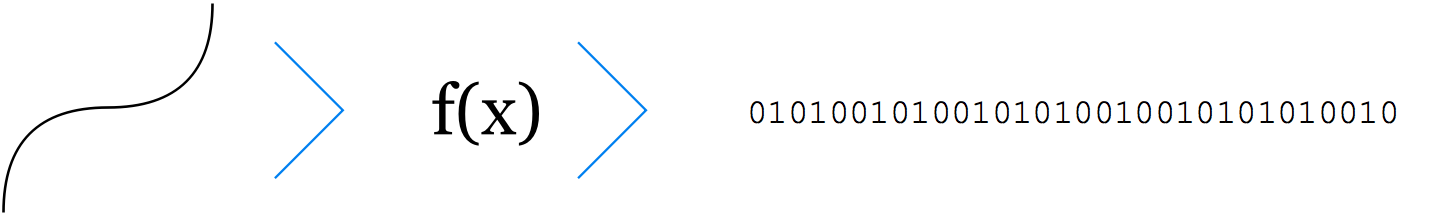
\includegraphics[width=0.8\linewidth]{images/primitive_encoding.png}
    \caption{Deciding upon an encoding scheme for vector primitives was one of the first decisions the group had to make.}
    \label{fig:primitive_encoding}
\end{figure}

Each primitives type is identified by the eight first bits.
To store a position on the screen, 32 bits is required: 16 bit for X and 16 bit for Y. // TODO: Reference discussion/result on why this is a limiting factor.
A line is represented by a start point and an end point.
To represent a quadratic Bézier curve a total of three points are needed, a start point, a control point and an end point.
The cubic Bézier curve includes one extra control point compared to the quadratic curve.
Table \ref{tbl:primitives} illustrates how each primitive is encoded as a binary string.

With the basic primitives linear, quadratic, and cubic Bézier curves, most other shapes can be constructed.
A square can be represented as four lines, a circle as multiple Bézier curves, and so on.

\begin{table}[h]
    \centering
    \begin{tabular}{|l|l|l|l|l|l|l|l|l|l|}
    \hline
    Primitive type (8) & x (16) & y (16) & x (16) & y (16) & x (16) & y (16) & x (16) & y (16) & Total bits \\ \hline
    Linear Bézier    & \(p_0^x \) & \(p_0^y \) & \(p_1^x \) & \(p_1^y \) & ~   & ~   & ~   & ~   & 72    \\ \hline
    Quadratic Bézier & \(p_0^x \) & \(p_0^y \) & \(p_1^x \) & \(p_1^y \) & \(p_2^x \) & \(p_2^y \) & ~   & ~   & 104   \\ \hline
    Cubic Bézier     & \(p_0^x \) & \(p_0^y \) & \(p_1^x \) & \(p_1^y \) & \(p_2^x \) & \(p_2^y \) & \(p_3^x \) & \(p_3^y \) & 136   \\ \hline
    \end{tabular}
    \caption{Binary encoding of primitives. Bit size in parenthesis.}
	\label{tbl:primitives}
\end{table}

\subsection{Vector Images}

A vector image, or a scene, is a 2D canvas of fixed width and height on which primitives are places.
The \vthreek architecture represents a scene conceptually as a collection of primitives.
Since primitives are represented with 16-bit integer coordinate-components, scene dimension is $65535 * 65535$.
This conceptual representation maps to a 1024 word deep, 136 bit wide, dual port scene memory module implemented using block RAM \cite{xilinx-block-ram} on the FPGA.
Since the size of the scene memory is static, the architecture maintains a primitive counter, indicating how many primitives are actually in the scene at any given time.
